\chapter{Projektfindung}

    Zu Beginn des Projekts wurden wir von unserem Praxispartner mit drei Fragestellungen konfrontiert, unter denen wir uns für eine wählen konnten:

    \vspace{1em}
    \begin{tabular}{ l|p{13.5cm} }
        \quad & Wie lässt sich der Verkehr für Einkäufe und Lieferungen reduzieren, um die Schadstoffbelastungen in der Luft zu minimieren?
    \end{tabular}
    \\[1em]
    \begin{tabular}{ l|p{13.5cm} }
        \quad & Wie lässt sich die Müllentsorgung in der Innenstadt und in den Grünflächen optimieren (z.B. Roboter, automatische Mülltrennung, Füllstandsensoren etc.)?
    \end{tabular}
    \\[1em]
    \begin{tabular}{ l|p{13.5cm} }
        \quad & Wie lässt sich Informations- und Kommunikationstechnik (IKT) (Rechenzentren, WLAN, Breitband) für eine umwelt- und ressourcenschonende Stadtgestaltung (z.B. Abwärme der Rechenzentren) nutzen? 
    \end{tabular}
    \vspace{1em}

    Im Anschluss des KickOff-Veranstaltung haben wir uns für die zweite Frage, die das Thema Müllentsorgung thematisiert entschieden, da wir dabei die größten Freiheiten bei der Gestaltung des Prototyps gesehen haben und Lust hatten uns mit der Problematik auseinander zu setzen.

    In den 

    \begin{figure}[h]
        \begin{center}
            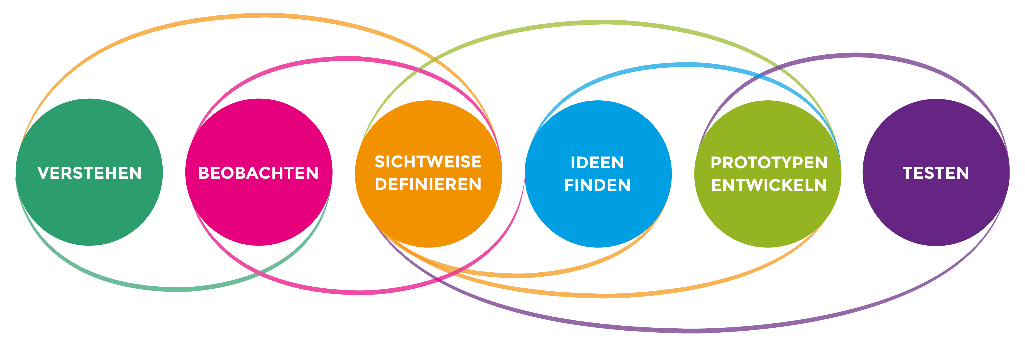
\includegraphics[width=11cm]{media/00_introduction/design_thinking_2.png}
        \end{center}
        \caption{Der Design-Thinking-Prozess\protect\footnote{Quelle: Design Thinking Workshop CrossInnovationClass}}
        \label{fig:dt_2}
    \end{figure}

    \begin{figure}[h]
        \begin{center}
            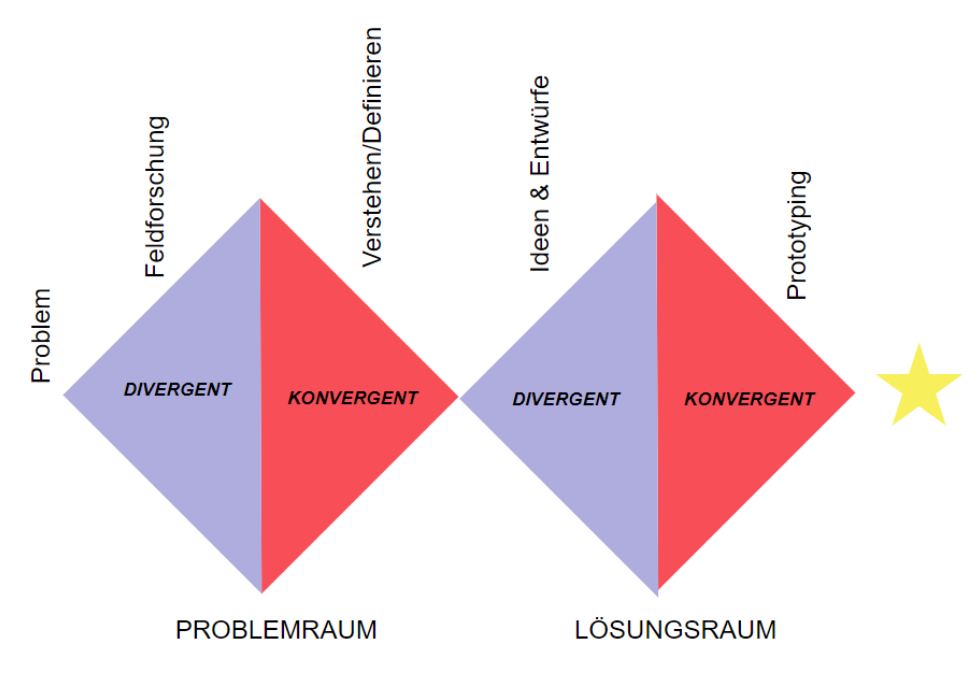
\includegraphics[width=10cm]{media/00_introduction/design_thinking_1.png}
        \end{center}
        \caption{Denkmodell \enquote{Double Diamond}\protect\footnotemark[\value{footnote}]}
        \label{fig:dt_1}
    \end{figure}


    \vspace{1em}
    \framebox[\textwidth]{
        \begin{minipage}{\textwidth-1em}
            \vspace{.4em}
            \textbf{Design Thinking}
            \\ \\
            
            Design Thinking ist ein Prozess zur Ideenfindung und -entwicklung.
            Dabei steht der Mensch im Mittelpunkt der mit einem Problem konfrontiert ist.
            
            Abbildung\,\ref{fig:dt_2} zeigt die sechs Phasen die im Prozess durchlaufen werden und visualisiert den iterativen Ansatz, das mehrmalige durchlaufen in unterschiedlichen Kreisen im Laufe des Prozess.\\

            In vielen Veranstaltungen der CIC ist uns besonders das Modell sdes \enquote{Double Diamonds} (Abbildung\,\ref{fig:dt_1}) begegnet, denn der Ablauf der Cross wurde in einem solchen Rahmen strukturiert.
            Anhand der Fragestellung wird ein breiter Problemraum geöffnet in dem möglichst viel Wissen aus verschiedenen Perspektiven zusammenfließt. Diese Problemdefinition wird nun konkretisiert, um einen Lösungsraum zu öffnen, der Lösungsansätze jeder Art zulässt.
            Anschließend werden auch diese im Team besprochen und am Ende entsteht ein konkreter Prototyp.
            \vspace{.4em}
        \end{minipage}
    }
    \vspace{1em}

        Design THinking einer aus drei, aber nicht ins Detail der anderen.
        
        Wie hat sich Skizze der Idee und der Realisierung

\chapter{Projektbeschreibung}
    
    Eingehendere Beschreibung der Projekt-Idee untermauert mit
    Skizzen/Zeichnungen

    \begin{figure}[h]
        \begin{center}
            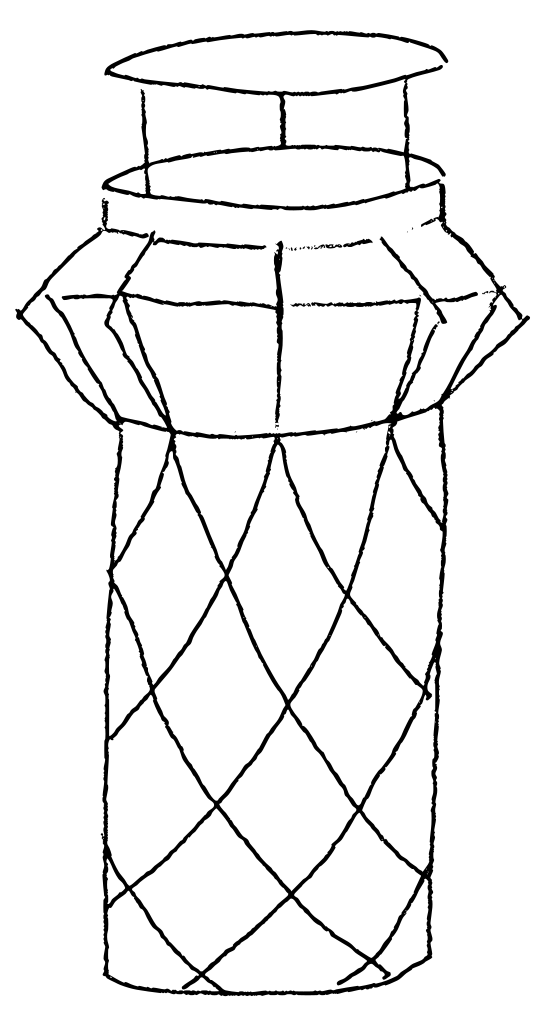
\includegraphics[width=5cm]{media/01_project/bin.png}
        \end{center}
        \caption{Skizze des Entwurfs mit Rautenmuster}
        \label{fig:bin_1}
    \end{figure}